\subsection{珠弹簧(bead-spring)模型}
另一类重要的理想链模型是所谓的珠弹簧模型,在这些模型中,沿粗粒链的连续粒子被“弹簧电势(spring potentials)”所束缚,这些弹簧电势有多种形式被选择。定义这些模型的势能$U_{0}$是最合适表达键向量的术语。因此,配分函数和相空间分布函数的$(N+1)$个粒子链(见图2.1)通常被写成公式(2.6)-(2.7)的形式。如果这样一个链的N键全部等价和没有外场的干扰,这些势能可以表示为:
\begin{equation}\label{2.26}
\begin{split}
U_{0}(\mathbf{b}^{N})= \sum_{i=1}^{N}h(|\mathbf{b}_{i}|)
\end{split}
\end{equation}
其中$h(x)$是沿高分子聚合物相邻粒子的弹簧电势,因此得出的结论是:
\begin{equation}\label{2.27}
Z_{0}=V(\int d\mathbf{b}~\exp[-\beta h(|\mathbf{b}|)])^N 
\end{equation}
\begin{equation}\label{2.28}
\begin{split}		
P_{0} (r_{0},\mathbf{b}^N) =V^{-1} \prod_{i=1}^{N} \frac{\exp[-\beta h(|\mathbf{b}_{i}|)]}{\int d \mathbf{b}_{i}~\exp[-\beta h(|\mathbf{b}_{i}|)]}
\end{split}
\end{equation}
因此,每个键向量$\mathbf{b}_{i}$都是独立分布的,其统计权重与$\exp[-\beta h(|\mathbf{b}_{i}|)]$成正比。 

它仍然需要指定键h弹簧电势的函数形式。最常见的选择是定义所谓的离散高斯链模型的谐波键电势(harmonic bond potential): 
\begin{equation}\label{2.29}
h(x)=\frac{3k_{B}T}{2b^2} x^2  
\end{equation}
这个电势的参数b,可以被理解为键的均方根长度,因为对任意键i 
\begin{align}\label{2.30}
\begin{split}
<\mathbf{b}_{i}.\mathbf{b}_{i}>_{0}&= \frac{\int_{-\infty}^{\infty} d\mathbf{b}_{i}(\mathbf{b}_{i}.\mathbf{b}_{i})~\exp[-\beta h(|\mathbf{b}_{i}|)])}{\int_{-\infty}^{\infty} d\mathbf{b}_{i}~e^[-\beta h(|\mathbf{b}_{i}|)]}\\ &=\frac{\int_{-\infty}^{\infty}dx_1\int_{-\infty}^{\infty}dx_2\int_{-\infty}^{\infty}dx_3(x_1^2+x_2^2+x_3^2)e^{-\frac{3}{2b^2}(x_1^2+x_2^2+x_3^2)}}{\int_{-\infty}^{\infty}dx_1\int_{-\infty}^{\infty}dx_2\int_{-\infty}^{\infty}dx_3~e^[-\frac{3}{2b^2}(x_1^2+x_2^2+x_3^2)]}\\ &=\frac{3\int_{-\infty}^{\infty}dx_1\int_{-\infty}^{\infty}dx_2\int_{-\infty}^{\infty}dx_3~x_1^2e^[-\frac{3}{2b^2}(x_1^2+x_2^2+x_3^2)]}{\int_{-\infty}^{\infty}dx_1\int_{-\infty}^{\infty}dx_2\int_{-\infty}^{\infty}dx_3~e^[\frac{-3}{2b^2}(x_1^2+x_2^2+x_3^2)]}\\ &=\frac{3 \times\frac{1}{2} (\frac{2b^2}{3})^{3/2}\sqrt{\pi}}{(\frac{2b^2\pi}{3})^{\frac{1}{2}}}\\ &=b^2
\end{split}
\end{align}
其中,所需的高斯积分是附录B中给出的公式的。

离散高斯链的均方端到端向量可以类似的计算,特别的:
\begin{equation}\label{2.31}
<\mathbf{R}\cdot\mathbf{R}>_{0}=\sum_{i=1}^{N}\sum_{i=1}^{N}<\mathbf{b}_{i}\cdot\mathbf{b}_{i}>_{0}
\end{equation}
在这个表示当中,当$i\neq j$时,独立分布的键向量不存在,当$i\neq j$时,$<\mathbf{b}_{i}\cdot\mathbf{b}_{j}>_{0}=<\mathbf{b}_{i}>_{0}<\mathbf{b}_{j}>_{0}=0$。因此
\begin{equation}\label{2.32}
<\mathbf{R}\cdot\mathbf{R}>_{0}=N<\mathbf{b}_{i}\cdot\mathbf{b}_{i}>_{0}=Nb^2
\end{equation}
并精确的恢复了公式(2.12)的理想链标度,$R=bN^\frac{1}{2}$,除了将b作为自由连接模型固定键长与离散高斯模型的均方根外,我们发现这两个理想模型均方端到端向量的表达是一致的。这容易证明回璇半径$R_{g}$是等价的。因此公式(2.16)也可以适用离散高斯链。
\begin{figure}[H]
\centering
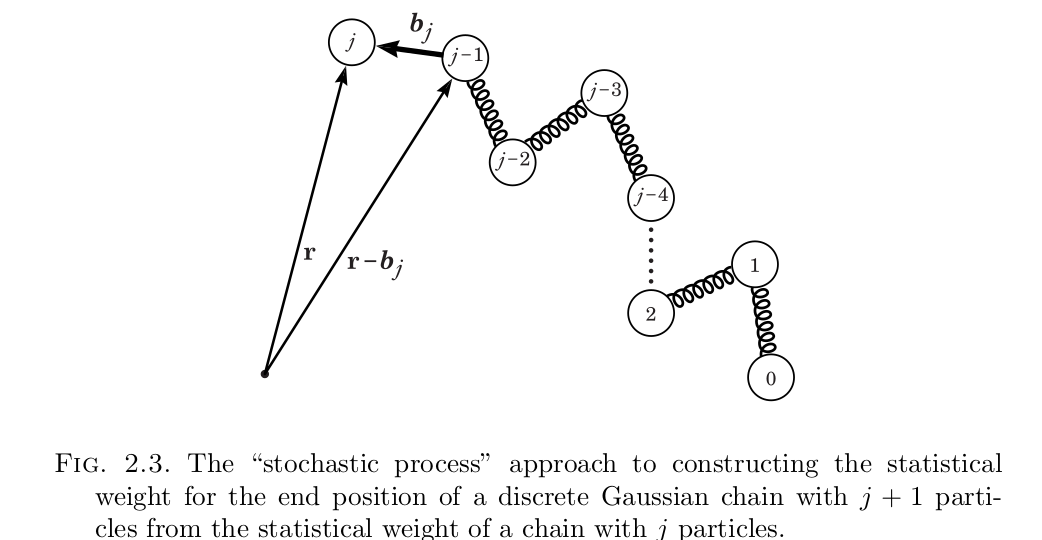
\includegraphics[width=15cm]{./figures/23.png}
\caption{"随机过程”方法构造离散高斯链的末端的统计权重,其中j+1粒子来自j粒子的统计权重。}
\label{figures23}
\end{figure}


为了更充分的探索自由链接和离散高斯链模型的关系,利用随机过程的联系是非常有用的。关于自由连接链,我们考虑约化分布函数$P_{0}(\mathbf{r},j)$,表示在r位置观察(j+1)--粒子链末端粒子j的概率密度。假设一条链的概率密度比它少一个粒子$p_{0}(\mathbf{r},j-1)$,如图\ref{figures23}所示,通过Chapman-Kolmogorov公式建立:
\begin{equation}\label{2.33}
P_{0}(\mathbf{r},j)=\int d\mathbf{b}_{j} \varPhi (\mathbf{b}_{j};\mathbf{r}-\mathbf{b}_{j})~p_{0}(\mathbf{r}-\mathbf{b}_{j},j-1)
\end{equation}
在这个表达式中$\varPhi (\mathbf{b}_{j};\mathbf{r}-\mathbf{b}_{j})$是连续粒子j和j-1键向量假设在$\mathbf{b}_{j}$的条件概率密度,给出粒子j-1在$\mathbf{r}-\mathbf{b}_{j}$位置。这是规范化的,因此$\int d\mathbf{b}_{j} \varPhi (\mathbf{b}_{j};\mathbf{r}-b\mathbf{b}_{j})=1$。不在任何外场的离散高斯链,$\varPhi$是链上粒子指数j(即随机过程是“平稳的”)和起始位置$\mathbf{r}-\mathbf{b}_{j}$上独立,因此,条件转移概率密度只反映键位移的高斯分布:
\begin{equation}\label{2.34}
\begin{split}
\begin{aligned}
\varPhi(\mathbf{b}_{j};\mathbf{r}-\mathbf{b}_{j})=\varPhi(\mathbf{b}_{j})&=\frac{\exp[-\beta h(|\mathbf{b}_{j}|)]}{\int d\mathbf{b}_{j}~\exp[-\beta h(|\mathbf{b}_{j}|)]} \\ &=(\frac{3}{2 \pi b^2})^{\frac{3}{2}}~\exp[-3|\mathbf{b}_{j}|^2 / (2b^2)]
\end{aligned}
\end{split}
\end{equation}
公式(\ref{2.33})易于用Fourier变换求解,因为离散高斯链$\varPhi$转移概率形式意味着右边是一个三维的卷积积分公式(见附录A)。因此公式(\ref{2.33})的Fourier变换得到Fourier变换的乘积
\begin{equation}\label{2.35}
\hat{p}_{0}(\mathbf{k},j)=\hat{\varPhi}(\mathbf{k})\hat{p}_{0}(\mathbf{k},j-1)
\end{equation}
对$j=1,2,\dots ,N$归纳递推得:
\begin{equation}\label{2.36}
\hat{p}_{0}(\mathbf{k},N)=[\hat{\varPhi}(\mathbf{k})]^N\hat{p}_{0}(\mathbf{k},0)
\end{equation}
公式(\ref{2.34})中的高斯转移概率的Fourier变换是高斯的$^{11}$。$\hat{\varPhi}(\mathbf{k})=\exp(-b^2|\mathbf{k}|^2/6)$,因此公式(\ref{2.36})的离散高斯链可以化简为:
\begin{equation}\label{2.37}
\hat{p}_{0}(\mathbf{k},N)=\exp(-R_{g}^2|\mathbf{k}|^2)\hat{p}_{0}(\mathbf{k},0)
\end{equation}
这里写$R_{g}=\sqrt{Nb^2/6}$作为链的回旋半径来计算,最后,我们专门讨论粒子0约束原点$p_{0}(\mathbf{r},0)=\delta(\mathbf{r})$的情况。其中$\hat{p}_{0}(\mathbf{k},0)=1$,则公式(\ref{2.37})的Fourier逆变换可以写成:
\begin{equation}\label{2.38}
p_{0}(\mathbf{R},N)=[3/(2\pi Nb^2)]^\frac{3}{2}\exp[-3|\mathbf{R}|^2/(2Nb^2)]
\end{equation}

将离散高斯链的这些结果和自由连接链的结果进行比较是很有意思的,特别的,我们发现自由连接链模型公式(2.21)的精确分布函数$\hat{p}_{0}(k,N)$的Fourier变换与离散高斯链公式(\ref{2.37})不一致,但是对于长度超过b,如:$b|k|<<1$,
\begin{equation}\label{2.39}
[j_{0}(b|\mathbf{k}|)]^N\approx [1-b^2|\mathbf{k}|^2/6+\dots]^N\approx \exp(-R_{g}^2|\mathbf{k}|^2)
\end{equation}
这两个函数是一致符合的。观察的结果是离散高斯链公式(\ref{2.38})是精确的,但是对于自由链接链的结果是近似的(要求$N>>1$且$|\mathbf{R}|<<Nb$)。

离散高斯连模型只是众多可设计的珠弹簧模型之一。这是个特别方便的模型,因为在粗粒键和介观端到端向量的水平上都是高斯的段分布,这便于分析计算各种各样单链的性能。然而,利用连接键的调和势(harmonic potential)的线性(Hookian)弹簧模型有时是不够的。例如:高斯链模型在描述低盐条件下(Netz and Orland,1999)的电解质时,可以表示较大的非物质拉伸。具有延伸特性强的流体力学流动作用下的高斯链也不能代表真实聚合物的无限延伸(Larson,1986)。在这种情况下,可以利用非线性的弹簧模型来防止非物质的扩展链现象。自由连接链也可以被应用,但是由于与固定键长度相关的完整性约束在动态高分子聚合物方案中往往更难实现。(Doi and Edwards,1986).

大部分非均匀聚合物的计算是通过数值计算的观点来实现的,目前使用非线性的珠弹簧模型比较容易,特别是公式(\ref{2.36})适用于所有键相同且其特点是仅取决于键长x的弹簧电势h(x)的任何珠弹簧。$\varPhi(\mathbf{k})$的形式是区分不同链模型的统计特征。一般情况下h(x)的转移概率密度的Fourier变换可以被写为:
\begin{equation}\label{2.40}
\hat{\varPhi(\mathbf{k})}=\frac{\int_{0}^{\infty} dx x^2j_{0}(|\mathbf{k}|x)\exp[-\beta h(x)]}{\int_{0}^{\infty} dx x^2\exp[-\beta h(x)]} 
\end{equation}
对于公式(2.29)的线性(高斯)弹簧模型$\hat{\varPhi(k)}=exp(-b^2|k|^2/6)$。比较公式(2.21)和(\ref{2.36})表明自由连接链模型可以类似的表示:$\hat{\varPhi_{FJ}(k)}=j_{0}(b|k|)$。

作为非线性的珠弹簧模型的例子,考虑类似流变学的计算Warner spring的电势:
\begin{equation}\label{2.41}
h(x)=\frac{2k_{B}T}{2b^2}\frac{x^2}{(1-x^2/b_{0}^2)}
\end{equation}
此电势包含的参数$b_{0}>0$即当$h(x)\to +\infty,x\to b_{0}$键的最大长度,但是,对于弱键的扩张$x/b_{0}<<1$公式(\ref{2.41})减到公式(\ref{2.29})中给定的调和键位电势。因此公式(\ref{2.41})是双参数非线性弹簧定律。它与离散高斯链模型中小键位移的线性定律一致。然而,对于强作用力键长在有限的$b_{0}$处是饱和的。

当被替换公式(\ref{2.40})时,公式(\ref{2.41})的非线性性弹簧模型会导致转换后的转移概率密度$\varPhi_{NL}(k)$可以表示为(wavevector)波矢量和无尺度$b/b_{0}$比的函数,对于$b/b_{0}<0.1$,$\varPhi_{NL}(b|k|,b/b_{0})$与线性弹簧函数$\varPhi_{G}(k)$几乎没差别。 然而,当$b/b_{0}$的值比较大时,非线性弹簧在波矢量中的影响依赖于$\varPhi_{NL}(k)$。图\ref{figures24}比较了离散高斯链、自由连接链和公式(\ref{2.41})的非线性珠弹簧链在$b/b_{0}=1$情况下的转移概率的Fourier变换。非线性弹簧定律对$|k|$具有振幅依赖性,其性质上类似于自由连接链。然而,自由链接模型振幅受到更强的阻尼,其键的长度被严格地约束为b。
\begin{figure}[H]
\centering
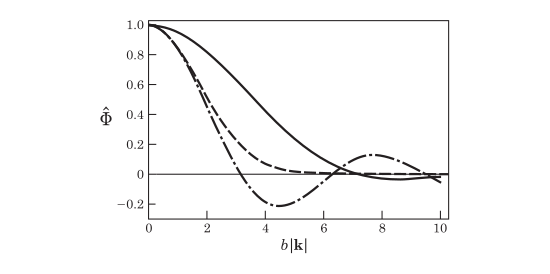
\includegraphics[width=15cm]{./figures/24.png}
\caption{分别是离散高斯(虚线),自由连接链(点虚线)和非线性弹簧模型(实线)的键转移概率$\varPhi_{G}$、$\varPhi_{Fj}$和$\varPhi_{NL}$的Fourier变换,用$b/b_{0}=1$来计算非线性弹簧模型}
\label{figures24}
\end{figure}
